\documentclass[conference]{IEEEtran}
\IEEEoverridecommandlockouts
\usepackage{cite}
\usepackage{amsmath,amssymb,amsfonts}
\usepackage{algorithmic}
\usepackage{graphicx}
\usepackage{textcomp}
\usepackage{xcolor}
\usepackage{bmpsize}
\usepackage{balance}

\def\BibTeX{{\rm B\kern-.05em{\sc i\kern-.025em b}\kern-.08em
    T\kern-.1667em\lower.7ex\hbox{E}\kern-.125emX}}
\begin{document}

\title{Malware detection based on performance counters}

\DeclareRobustCommand*{\IEEEauthorrefmark}[1]{\raisebox{0pt}[0pt][0pt]{\textsuperscript{\footnotesize\ensuremath{
 \ifcase#1\or {*}\or {**}\or {{**}*}\or {{**}{**}}\or 5\or 6\or 7\or 8 \else\textsuperscript{\expandafter\romannumeral#1}\fi}}}}

\author
{
 \IEEEauthorblockN
 {
   Omar Mohamed\IEEEauthorrefmark{1}
 }
 \IEEEauthorblockN
 {
  Ciprian-Bogdan Chirila\IEEEauthorrefmark{2}
 }
 \IEEEauthorblockA
 {\IEEEauthorrefmark{1}University ..., Turkey\\
  \IEEEauthorrefmark{2}University Politehnica of Timi\c{s}oara, Romania\\
  Department of Computers and Information Technology\\
  E-mail:
	omarmostafa1101@gmail.com; 
	chirila@cs.upt.ro
 }
}

\maketitle

\begin{abstract}
\end{abstract}

%\begin{keywords} 
%malware;
%performance counters;
%operating systems;
%program behaviour;
%clustering;
%\end{keywords}

\section{Introduction}
\label{sec:introduction}
...
In this paper we present a framework for training and evaluating models that detects malware in operating systems based on performance counters.

\cite{xAPI2019}

In Figure \ref{fig:approach} we present conceptually our approach.
\begin{figure}[!ht]
\centering
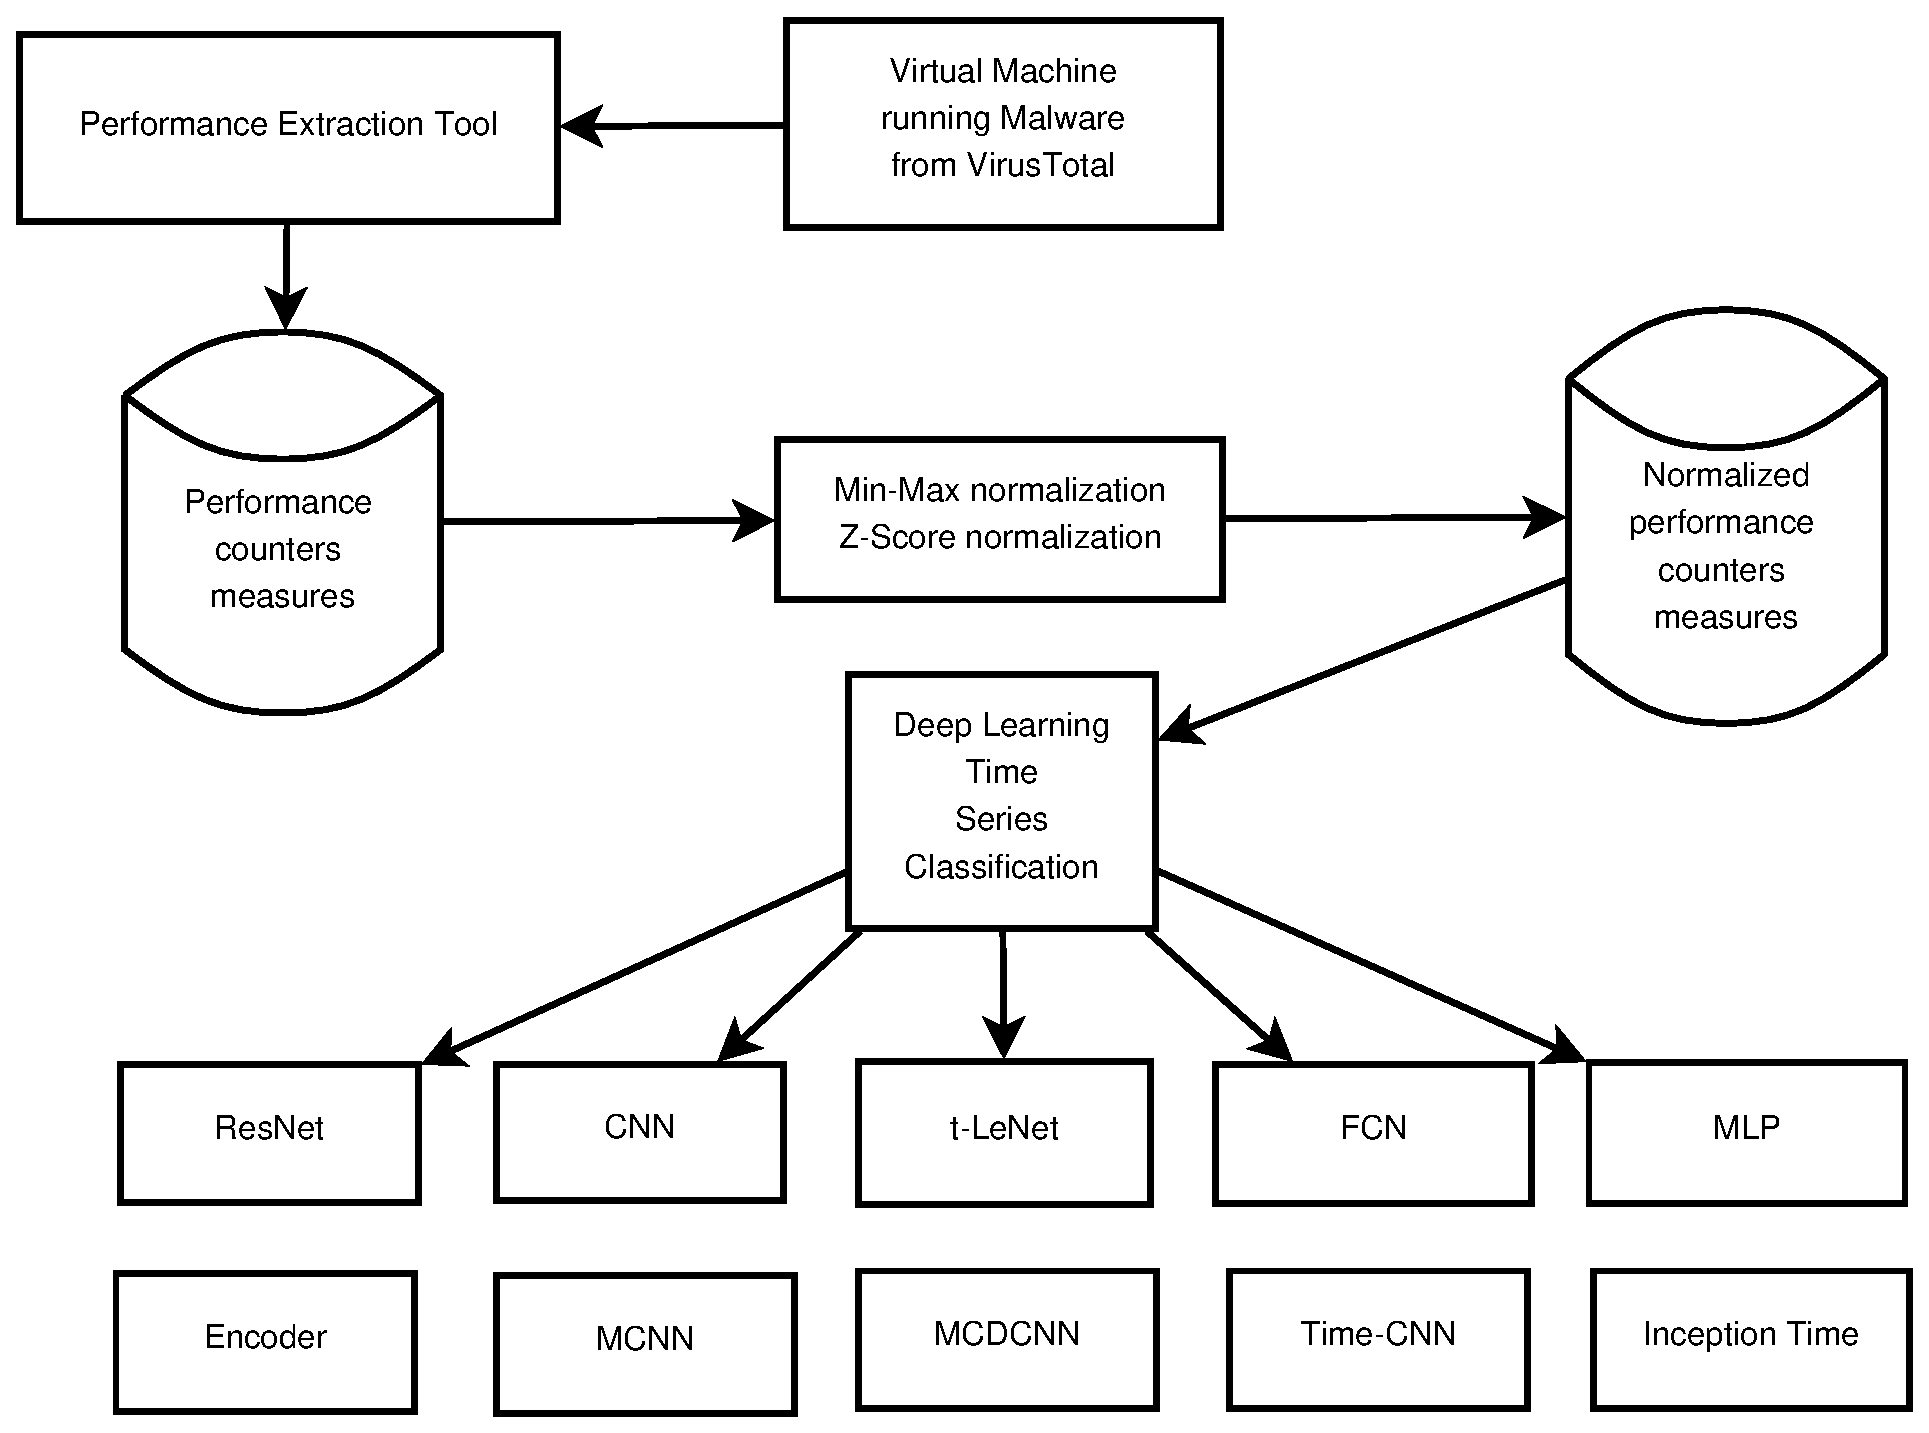
\includegraphics[width=8.5cm]{fig-approach.eps}
\caption{}
\label{fig:approach}
\end{figure}

We start our approach at a Virtual Machine (VM) running viruses from VirusTotal.
On the same VM we run a tool that collects the performance counters into several time series.
Next, the results are normalized using statistical operators like Min-Max and Z-Score.
On the resulted time series we trained several classification models:
i) ResNet;
ii) CNN;
iii) t-LeNet;
iv) FCN;
v) MLP;
vi) Encoder;
vii) MCNN;
viii) MCDCNN;
ix) Time CNN;
x) Inception Time.
On the trained classification models accuracy tests were performed and corresponding graphs were plotted.

We consider that the trained classfiers could be used on a real machine as a malware detection tool.

% paper structure
The paper is structured as follows.
Section \ref{sec:related-works} presents related works in the field of program behaviour analysis and performance counters.
Section \ref{sec:experimental-setup} presents the design of the performance counters extration tool and the configuration of the classification models.
Section \ref{sec:experimental-results} presents the experimental results from the trained classfication models.
Section \ref{sec:discussion} analyzes the experimental results. 
Section \ref{sec:conclusions-and-future-work} concludes and sets the future work.

\section{Related Works}
\label{sec:related-works}


\section{Experimental setup}
\label{sec:experimental-setup}


\section{Experimental results}
\label{sec:experimental-results}


\section{Discussion}
\label{sec:discussion}


\section{Conclusions and Future Work}
\label{sec:conclusions-and-future-work}
In this paper we presented an experimental setup where performance counters time series were extracted from a malware infected virtual machine.
The performance counter time series were normalized and were used to train 10 classification models.

As future work we intend to experiment with the 10 classifiers detecting malware and assessing their performance.

\bibliographystyle{plain}
\balance
\bibliography{bibliography}
\end{document}
